\documentclass[10pt,a4paper]{article}
\usepackage[utf8]{inputenc}
\usepackage[english]{babel}
\usepackage[T1]{fontenc}
\usepackage{amsmath}
\usepackage{amsfonts}
\usepackage{amssymb}
\usepackage{lmodern}
\usepackage{fancyvrb}
\usepackage{dirtree}
\usepackage{indentfirst}
\usepackage{listings}

%\usepackage{dot2texi}
\usepackage{tikz}
\usetikzlibrary{shapes,arrows}

\newcommand{\version}{\IfFileExists{../../version.txt}
{\input{../../version.txt}}
{\input{../../../version.txt}}
}

\newcommand{\command}[1]{%
\indent \fcolorbox{black}{white}{%
   \begin{minipage}{\dimexpr\textwidth-\parindent\relax}%
      #1
   \end{minipage}%
}
}

\newsavebox{\FVerbBox}
\newenvironment{sample}
{\par \vspace{0.2cm} \begin{lrbox}{\FVerbBox}
\begin{minipage}{\dimexpr\textwidth-\parindent\relax}}
{\end{minipage}
\end{lrbox}
\fcolorbox{black}{lightgray}{\usebox{\FVerbBox}}
\vspace{0.2cm}}

\newenvironment{sampletitle}
{\vspace{0.2cm} \noindent\textbf{Example} :
\begin{sample}}
{\end{sample}}

\newcommand{\samplecomment}[1]{%

\textit{#1}
}

\newcommand{\seealso}[1]{\vspace{0.2cm} \noindent\textbf{See also} :\par #1}

% tikz
\usetikzlibrary{calc}
\usetikzlibrary{arrows}
\usetikzlibrary{shadows}

\tikzset{block/.style={draw, text centered, fill=gray!10,drop shadow}}
\tikzset{connect/.style={draw, line width=1 pt}}

\author{Sebastien CAUX}
\title{GPStudio Tutorial \version : \\ 2. How to create and use a simple node project in command line mode?}

\begin{document}
\maketitle
\section{Introduction}
This tutorial is done to show how GPStudio is simple to use when you are using only IP in library on a supported board. The objective is to understand the basics of GPStudio tools and especially the command line tools. For this example, we use the famous Dreamcam platform, the first platform supported by GPStudio.\\

In this tutorial, we create a project for a specific platform and configure it. After that, we add some process in the project, setting up and connect it to image sensor and communication. Finally, we configure the smart camera with the compiled project and check results of processing on the viewer interface. \\

In a second time, we will create a custom process block externally configurable and test it on a real camera. \\

At the end of this tutorial, we will be able to use GPStudio with all the command line tools.

\section{Driving the flow from image sensor to USB}

\begin{figure}[h!]
\centering

\begin{tikzpicture}[node distance=8cm]

\tikzset{blocstyle/.style={block,rectangle,minimum height=1.8cm,text width=3cm}};

% blocks
\node[blocstyle] (bloc1) {\textbf{Image sensor}};
\node[blocstyle] (bloc2) at (7,0) {\textbf{Communication}};

% Flow to
\path[connect,->] (bloc1.east) -- node[above,pos=0.2]{out} node[above,pos=0.85]{in} (bloc2.west);

\end{tikzpicture}
\caption{Simple connection from image sensor to communication block, first step}
\end{figure}

\subsection{Create the project and configure platform}

At the very beginning, check if your tools are well installed by simply launch:
\begin{sample}
> gpnode $--$version \\
\# gpnode command line tool to manage a gpstudio node (\version)
\end{sample}

If you do not have this result, you probably need to set your PATH system variable or to call the setenv script. Read the first tutorial to do it.\\

Firstly, you need to create the project in an empty directory:
\begin{sample}
> mkdir tuto1\\
> cd tuto1\\
> \textbf{gpnode newproject} -n tuto1
\end{sample}

After that, you should have a file named \emph{tuto1.node} in the current directory. This file is the project file and contain the definition of the node. A node in GPStudio is a physical node, it can be a smart camera or a sensor. You can have only one project file per directory and gpnode always works on the project in the current directory. The directory name can be different that the project name, but you should not modify the name of the project file.\\

The next thing to do is to specify the platform that you want to use for this project. You can do it with:

\begin{sample}
> \textbf{gpnode setboard} -n dreamcam\_c3
\end{sample}

`dreamcam\_c3' corresponds to a DreamCam platform with Cyclone III FPGA. The board support package for the `dreamcam\_c3' camera is located at:

\emph{<gps-root>/support/board/dreamcam\_c3/dreamcam\_c3.dev}

DreamCam is now set as a target platform. You can check that with the command command{showboard}:

\begin{sample}
> \textbf{gpnode showboard}
\begin{Verbatim}
dreamcam_c3
\end{Verbatim}
\end{sample}

To have the complete list of supported board, use the gplib tool with the command \textbf{listboard}:

\begin{sample}
> \textbf{gplib} \textbf{listboard}
\begin{Verbatim}
arrow_sockit de0nano dreamcam_c3 stratixcam_s4
\end{Verbatim}
\end{sample}

\subsection{Add IO support that you need}
Until now, we only specify the Dreamcam as platform, but it is a modular one, you can use different types of image sensor and communication. We need to define witch one we want to use by adding the support of theses peripherals. \\

You can use this command to know the available devices for the platform that you have specified before:
\begin{sample}
> \textbf{gpnode listavailabledevice}
\begin{Verbatim}
led mt9 e2v ethernet usb
\end{Verbatim}
\end{sample}

For image sensor, you have two possibilities, mt9 from Aptina or e2v. For this example, we choose mt9:

\begin{sample}
> \textbf{gpnode adddevice} -n mt9
\end{sample}

By adding mt9 IO, gpnode fetches the name of the driver to use with this IO and copies the hardware driver files implementation. Like that, it allows you to use this image sensor in order to acquire pictures.\\

Now, to enable a communication, you have the choice between Ethernet or USB. Choose USB support:

\begin{sample}
> \textbf{gpnode adddevice} -n usb
\end{sample}

You can view the list of ios supports with the command \textbf{showio}:

\begin{sample}
> \textbf{gpnode showdevice}
\begin{Verbatim}
ios :
  + mt9 [mt9]
  + usb [usb_cypress_CY7C68014A]
\end{Verbatim}
\end{sample}

\subsection{Connect block flow}
To obtain a simple image sent from the image sensor to USB communication, we need a direct connection between `mt9' output image flow and `usb' input flow. To see flows that could be connected of a block, use the command \textbf{showblock} with a filter for looking only flows:

\begin{sample}
> \textbf{gpnode showblock} -n mt9 -f flows
\begin{Verbatim}
flows :
    -------------       
    |    mt9    |  out (8) 
    |           |---------->
    -------------
\end{Verbatim}
\end{sample}

And for usb block:

\begin{sample}
> \textbf{gpnode showblock} -n usb -f flows
\begin{Verbatim}
flows :
           -------------        
  in0 (8)  |           |  out0 (8)  
---------->|           |----------->
  in1 (8)  |           |  out1 (8)  
---------->|           |----------->
  in2 (8)  |    usb    |        
---------->|           |        
  in3 (8)  |           |        
---------->|           |        
           -------------
\end{Verbatim}
\end{sample}

So we want to have this graph of connection:
\begin{figure}[h!]
\centering
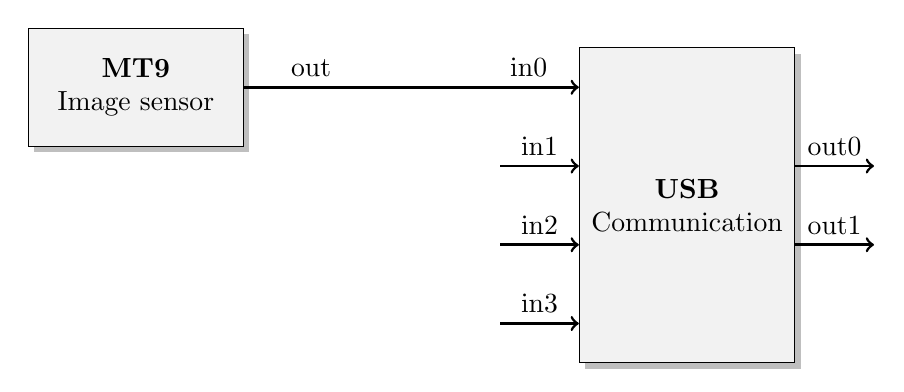
\begin{tikzpicture}[node distance=8cm]

\tikzset{blocstyle/.style={block,rectangle,minimum height=1.5cm,text width=2.5cm}};

% blocks
\node[blocstyle] (bloc1) {\textbf{MT9}\\Image sensor};
\node[blocstyle,minimum height=4cm] (bloc2) at (7,-1.5) {\textbf{USB}\\Communication};

% Flow to
\path[connect,->] (bloc1.east) -- node[above,pos=0.2]{out} node[above,pos=0.85]{in0} ([yshift=1.5cm]bloc2.west);
\path[connect,<-] ([yshift=0.5cm]bloc2.west) -- node[above]{in1} ++(-1,0);
\path[connect,<-] ([yshift=-0.5cm]bloc2.west) -- node[above]{in2} ++(-1,0);
\path[connect,<-] ([yshift=-1.5cm]bloc2.west) -- node[above]{in3} ++(-1,0);

\path[connect,->] ([yshift=0.5cm]bloc2.east) -- node[above]{out0} ++(1,0);
\path[connect,->] ([yshift=-0.5cm]bloc2.east) -- node[above]{out1} ++(1,0);

\end{tikzpicture}
\caption{Details on flow connexion}
\end{figure}

To do it, you need to add a connection with the command \textbf{connect}:
\begin{sample}
> \textbf{gpnode connect} -f mt9.out -t usb.in0
\end{sample}

To check effective connections, it is possible to print the list of connection with \textbf{showconnect}:
\begin{sample}
> \textbf{gpnode showconnect}
\begin{Verbatim}
connects:
  + mt9.out -> usb.in0 (msb)
\end{Verbatim}
\end{sample}

Your project is now fully configured. The next step is to generate code dedicated to the platform. We do it in a `build' subdirectory:

\begin{sample}
> \textbf{gpnode generate} -o build
\end{sample}

After that, a subdirectory `build' is created in your project directory with the following files:

\begin{figure}[h]
\dirtree{%
.1 tuto1/.
   .2 tuto1.node\DTcomment{project file}.
   .2 Makefile\DTcomment{Helper Makefile to call the built Makefile}.
   .2 \bfseries build/\DTcomment{output directory}.
        .3 top.vhd\DTcomment{generated top level}.
        .3 ci.vhd\DTcomment{generated CI block}.
        .3 pi.vhd\DTcomment{generated PI block}.
        .3 fi.vhd\DTcomment{generated FI block}.
        .3 node\_generated.xml\DTcomment{definition of the internal node}.
        .3 Makefile\DTcomment{Makefile}.
        .3 Makefile.local\DTcomment{paths for Makefile}.
        .3 params.h\DTcomment{addresses of each internal registers}.
        .3 \bfseries IP/ \DTcomment{local copy of used IPs}.
           .4 IP1.
           .4 IP2.
           .4 IP....
}
\caption{Files tree of the project and generated files}
\label{fig:archivetree}
\end{figure}

The produced Makefile offers you several commands:
\begin{itemize}
\item \textbf{generate}: regenerate the project if you made some modification
\item \textbf{compile}: launch the compiler for your platform and produce a bitstream for the FPGA
\item \textbf{send}: configure the connected camera with the bitstream
\item \textbf{view}: launch the viewer
\end{itemize}

To launch the compilation process, call make with the rule `compile'

\begin{sample}
> make compile
\end{sample}

After few minutes, your project is now compile and ready to send to the camera.

First of all, powered up the DreamCam. Then, connect an USB cable from your computer to the USB communication board at the rear of the camera. Connect a second one to the internal JTAG near the power board.

To configure the FPGA with the generated bitstream, use the `send' rule of the Makefile

\begin{sample}
> make send
\end{sample}

This command needs only few seconds to be done. If no errors appear, camera is ready and you can launch the debugger viewer to test your project, \textbf{gpviewer}. The \texttt{make view} command launch gpviewer with the \texttt{node\_generated.xml} file as argument. This file configure the interface. Let is try

\begin{sample}
> make view
\end{sample}

\begin{figure}[h!]
\centering
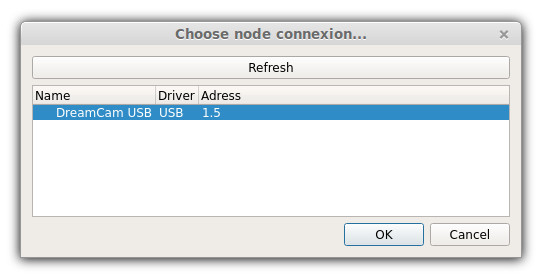
\includegraphics[scale=0.6]{gpviewer_connect_node.jpg}
\caption{First windows of gpviewer to choose your camera}
\end{figure}

gpviewer ask you which camera he need to open because it supports many camera with different types of connection at the same time.

\begin{figure}[h!]
\centering
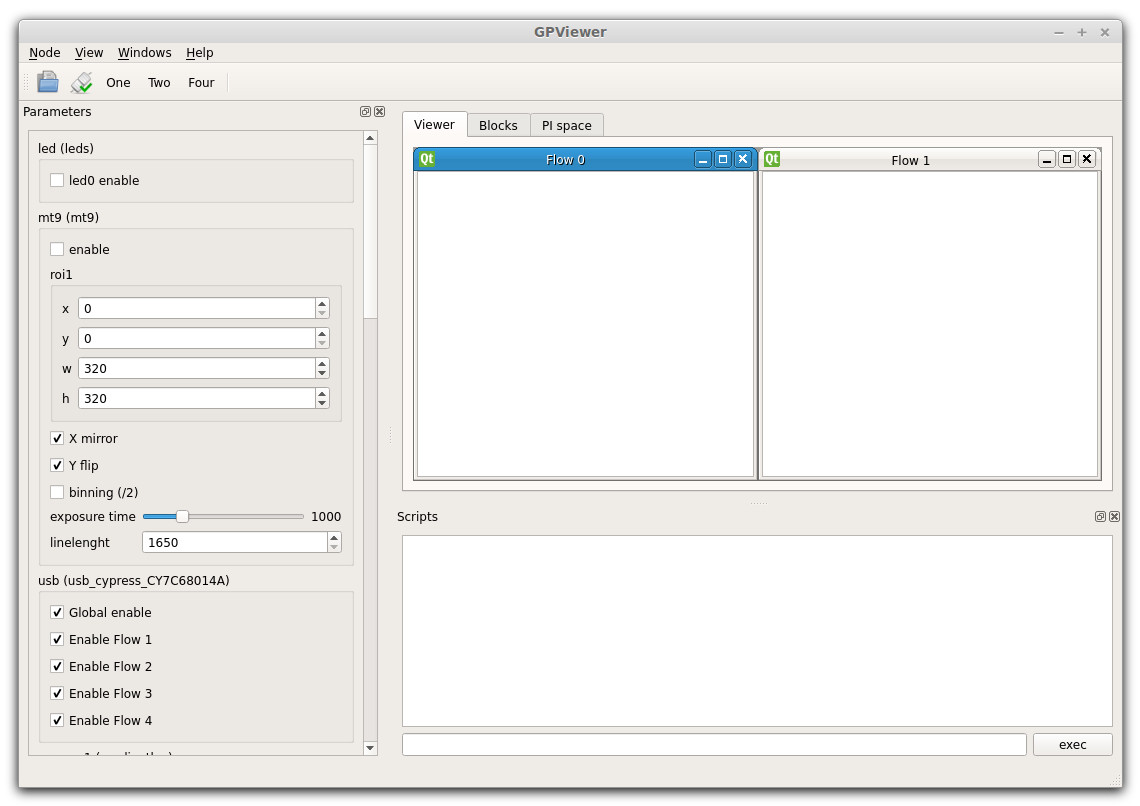
\includegraphics[scale=0.35]{gpviewer_mainwindows.jpg}
\caption{First windows of gpviewer to choose your camera}
\end{figure}

\newpage
\section{Adding a process from GPStudio library}
In this second part, we want to add some processing between the image sensor and the communication to obtain a smart camera and not only a `webcam'.

\begin{figure}[h!]
\centering
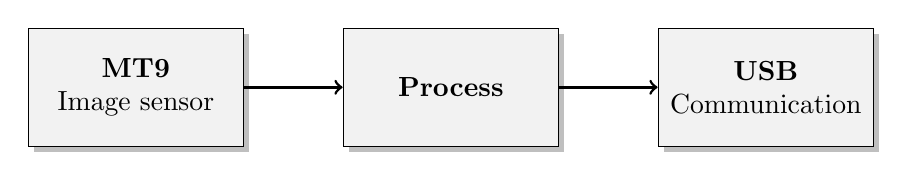
\begin{tikzpicture}[node distance=8cm]

\tikzset{blocstyle/.style={block,rectangle,minimum height=1.5cm,text width=2.5cm}};

% blocks
\node[blocstyle] (bloc1) {\textbf{MT9}\\Image sensor};
\node[blocstyle] (blocproc) at (4,0) {\textbf{Process}};
\node[blocstyle] (bloc2) at (8,0) {\textbf{USB}\\Communication};

% Flow to
\path[connect,->] (bloc1) -- (blocproc);
\path[connect,->] (blocproc) -- (bloc2);

\end{tikzpicture}
\caption{Details on flow connexion}
\end{figure}

\subsection{Add process that you need}
Check process that could be use

\begin{sample}
> \textbf{gplib listprocess}
\begin{Verbatim}
conv gradienthw histogramhw hog lbp normhw roi slidevm
\end{Verbatim}
\end{sample}

For example, we add a gradienthw as process block and we call it `process1'

\begin{sample}
> \textbf{gpnode addprocess} -n process1 -d gradienthw
\end{sample}

To have the list of process in the project, just type

\begin{sample}
> \textbf{gpnode showprocess}
\begin{Verbatim}
process :
  + process1 [gradienthw]
\end{Verbatim}
\end{sample}
  

\subsection{Connect process flow}

Take a look to the flow name of the process

\begin{sample}
> \textbf{gpnode showblock} -n process1 -f flows
\begin{Verbatim}
flows :
           ------------------
  in (16)  |                |  magnitude (16)
---------->|                |----------------->
           |    process1    |    angle (16)
           |                |----------------->
           ------------------
\end{Verbatim}
\end{sample}

\begin{figure}[h!]
\centering
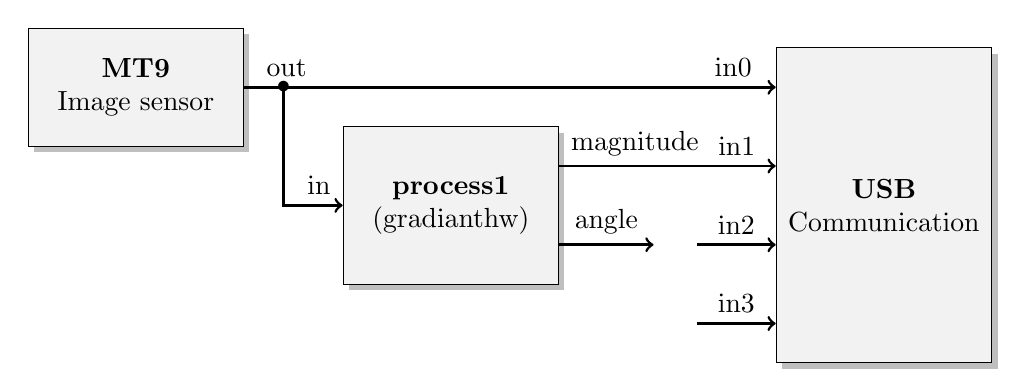
\begin{tikzpicture}[node distance=8cm]

\tikzset{blocstyle/.style={block,rectangle,minimum height=1.5cm,text width=2.5cm}};

% blocks
\node[blocstyle] (bloc1) {\textbf{MT9}\\Image sensor};
\node[blocstyle,minimum height=4cm] (bloc2) at (9.5,-1.5) {\textbf{USB}\\Communication};
\node[blocstyle,minimum height=2cm] (process1) at (4,-1.5) {\textbf{process1}\\(gradianthw)};

% Flow to
\path[connect,->] (bloc1.east) -- node[above,pos=0.08]{out} node[above,pos=0.92]{in0} ([yshift=1.5cm]bloc2.west);
\path[connect,->] ([yshift=0.5cm]process1.east) -- node[above,pos=0.35]{magnitude} node[above,pos=0.82]{in1} ([yshift=0.5cm]bloc2.west);
\path[connect,->] ([yshift=-0.5cm]process1.east) -- node[above]{angle} ++(1.2,0);
\path[connect,<-] ([yshift=-0.5cm]bloc2.west) -- node[above]{in2} ++(-1,0);
\path[connect,<-] ([yshift=-1.5cm]bloc2.west) -- node[above]{in3} ++(-1,0);

\path[connect,->] (bloc1.east) -- ++(0.5,0) node{$\bullet$} |- node[above,pos=0.8]{in} (process1);

\end{tikzpicture}
\caption{Details on flow connexion}
\end{figure}


\begin{sample}
> \textbf{gpnode connect} -f mt9.out -t process1.in\\
> \textbf{gpnode connect} -f process1.magnitude -t usb.in1
\end{sample}

\begin{sample}
> \textbf{gpnode showconnects}
\begin{Verbatim}
connects :
  + mt9.out -> usb.in0 (msb)
  + mt9.out -> process1.in (msb)
  + process1.magnitude -> usb.in1 (msb)
\end{Verbatim}
\end{sample}

\section{Creating simple custom process}
A tool is done to create custom block process, \textbf{gpproc}. It allows to describe interfaces of your process and provide a template to fill with your code. \\

As example, we will create a simple image threshold process with an input image and an output result.

\begin{figure}[h!]
\centering
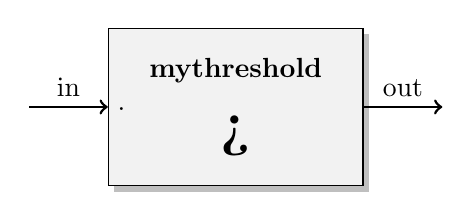
\begin{tikzpicture}[node distance=8cm]

\tikzset{blocstyle/.style={block,rectangle,minimum height=1.5cm,text width=2.5cm}};

% blocks
\node[blocstyle,minimum height=2cm,text width=3cm] (process1) {\textbf{mythreshold}\\ .\newline \textbf{\huge{>}}};

\path[connect,->] (process1.east) -- node[above]{out} ++(1,0);
\path[connect,<-] (process1.west) -- node[above]{in} ++(-1,0);

\end{tikzpicture}
\caption{Details on flow connexion}
\end{figure}

\subsection{Creating the process and defining the structure}

In your node directory, create a new directory with the process name and add a process project
\begin{sample}
> mkdir mythreshold \\
> cd mythreshold \\
> \textbf{gpproc new} -n mythreshold
\end{sample}

A new file with the \textit{.proc} will appear in the current directory. This file represents the block process definition.

Now, we can add flow interfaces input and output respectively named `in' and `out'
\begin{sample}
> \textbf{gpproc addflow} -n in -d in -s 8 \\
> \textbf{gpproc addflow} -n out -d out -s 8
\end{sample}

You can check that with \textbf{showblock} command
\begin{sample}
> \textbf{gpproc showblock}
\begin{verbatim}
          ---------------------           
  in (8)  |    mythreshold    |  out (8)  
--------->|                   |---------->
          ---------------------
\end{verbatim}
\end{sample}

Generate template in the directory hdl
\begin{sample}
> \textbf{gpproc generate} -o hdl \\
mythreshold.vhd generated \\
mythreshold\_process.vhd generated
\end{sample}

Two files are provided by the block template generator.

\begin{figure}[h!]
\centering
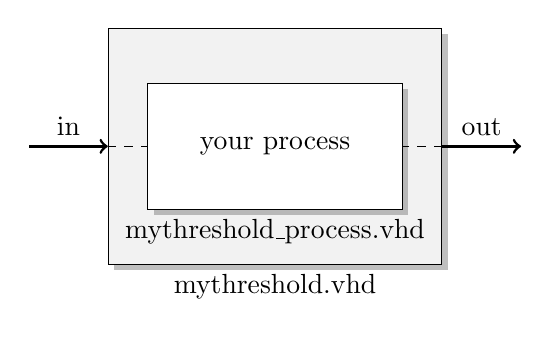
\begin{tikzpicture}[node distance=8cm]

\tikzset{blocstyle/.style={block,rectangle,minimum height=1.5cm,text width=2.5cm}};

% blocks
\node[blocstyle,minimum height=3cm,text width=4cm,label={below:mythreshold.vhd}] (process1) {};
\node[blocstyle,minimum height=1.6cm,text width=3cm,fill=white,label={below:mythreshold\_process.vhd}] (process1proc) {your process};

\path[connect,->] (process1.east) -- node[above]{out} ++(1,0);
\path[connect,<-] (process1.west) -- node[above]{in} ++(-1,0);

\path[draw,dashed] (process1.east) -- (process1proc);
\path[draw,dashed] (process1.west) -- (process1proc);

\end{tikzpicture}
\caption{Details on flow connexion}
\end{figure}

\texttt{mythreshold.vhd} content:
\lstset{language=VHDL,tabsize=3,rulecolor=\color{orange}}
\begin{lstlisting}[frame=single]
library IEEE;
use IEEE.STD_LOGIC_1164.all;
use IEEE.NUMERIC_STD.all;
library std;

entity threshold is
	generic (
		CLK_PROC_FREQ : integer;
		IN_SIZE       : integer;
		OUT_SIZE      : integer
	);
	port (
		clk_proc : in std_logic;

		------------------------- in flow -----------------------
		in_data  : in std_logic_vector(IN_SIZE-1 downto 0);
		in_fv    : in std_logic;
		in_dv    : in std_logic;

		------------------------ out flow -----------------------
		out_data : out std_logic_vector(OUT_SIZE-1 downto 0);
		out_fv   : out std_logic;
		out_dv   : out std_logic
	);
end threshold;

architecture rtl of threshold is
component threshold_process
	generic (
		CLK_PROC_FREQ : integer;
		IN_SIZE       : integer;
		OUT_SIZE      : integer
	);
	port (
		clk_proc : in std_logic;

		------------------------- in flow -----------------------
		in_data  : in std_logic_vector(IN_SIZE-1 downto 0);
		in_fv    : in std_logic;
		in_dv    : in std_logic;

		------------------------ out flow -----------------------
		out_data : out std_logic_vector(OUT_SIZE-1 downto 0);
		out_fv   : out std_logic;
		out_dv   : out std_logic
	);
end component;

begin
	threshold_process_inst : threshold_process
    generic map (
		CLK_PROC_FREQ => CLK_PROC_FREQ,
		IN_SIZE       => IN_SIZE,
		OUT_SIZE      => OUT_SIZE
	)
    port map (
		clk_proc => clk_proc,
		in_data  => in_data,
		in_fv    => in_fv,
		in_dv    => in_dv,
		out_data => out_data,
		out_fv   => out_fv,
		out_dv   => out_dv
	);

end rtl;
\end{lstlisting}

\texttt{threshold\_process.vhd} content :
\begin{lstlisting}[frame=single]
library IEEE;
use IEEE.STD_LOGIC_1164.all;
use IEEE.NUMERIC_STD.all;
library std;

entity threshold_process is
	generic (
		CLK_PROC_FREQ : integer;
		IN_SIZE       : integer;
		OUT_SIZE      : integer
	);
	port (
		clk_proc : in std_logic;

		------------------------- in flow -----------------------
		in_data  : in std_logic_vector(IN_SIZE-1 downto 0);
		in_fv    : in std_logic;
		in_dv    : in std_logic;

		------------------------ out flow -----------------------
		out_data : out std_logic_vector(OUT_SIZE-1 downto 0);
		out_fv   : out std_logic;
		out_dv   : out std_logic
	);
end threshold_process;

architecture rtl of threshold_process is

begin
	data_process : process (clk_proc, reset_n)
	begin
		if(reset_n='0') then
			out_data <= (others => '0');
			out_dv <= '0';
			out_fv <= '0';
		elsif(rising_edge(clk_proc)) then
			out_dv <= in_dv;
			out_fv <= in_fv;

			if(in_dv='1' and in_fv='1') then
				out_data <= in_data;
			end if;
		end if;
	end process;
end rtl;
\end{lstlisting}

By default, the generated process file is a by pass. Replace the copy of the input pixel value to the output by a conditional statement to binarise the picture in \texttt{threshold\_process.vhd}:
\begin{lstlisting}[frame=single]
	if(in_dv='1' and in_fv='1') then
		if(in_data<std_logic_vector(to_unsigned(127, IN_SIZE))) then
			out_data <= (others => '0');
		else
			out_data <= (others => '1');
		end if;
	end if;
\end{lstlisting}

Add generated files to the project
\begin{sample}
> \textbf{gpproc addfile} -p hdl/mythreshold.vhd -t vhdl -g hdl \\
> \textbf{gpproc addfile} -p hdl/mythreshold\_process.vhd -t vhdl -g hdl
\end{sample}

Return to the node project and add your process
\begin{sample}
> cd .. \\
> \textbf{gpnode addprocess} -n mythreshold1 -d mythreshold/mythreshold.proc
\end{sample}

Connect the input flow to the image sensor and the output to a free input flow of the USB communication block
\begin{sample}
> \textbf{gpnode connect} -f mt9.out -t mythreshold1.in \\
> \textbf{gpnode connect} -f mythreshold1.out -t usb.in2
\end{sample}

Like that, you obtain
\begin{figure}[h!]
\centering
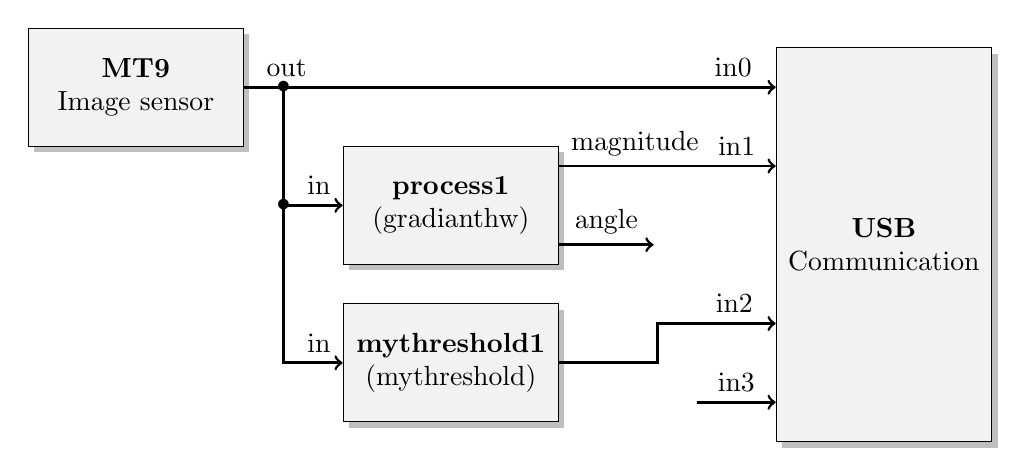
\begin{tikzpicture}[node distance=8cm]

\tikzset{blocstyle/.style={block,rectangle,minimum height=1.5cm,text width=2.5cm}};

% blocks
\node[blocstyle] (bloc1) {\textbf{MT9}\\Image sensor};
\node[blocstyle,minimum height=5cm] (bloc2) at (9.5,-2) {\textbf{USB}\\Communication};
\node[blocstyle,minimum height=1.5cm] (process1) at (4,-1.5) {\textbf{process1}\\(gradianthw)};
\node[blocstyle,minimum height=1.5cm] (mythreshold1) at (4,-3.5) {\textbf{mythreshold1}\\(mythreshold)};

% Flow to
\path[connect,->] (bloc1.east) -- node[above,pos=0.08]{out} node[above,pos=0.92]{in0} ([yshift=2cm]bloc2.west);
\path[connect,->] ([yshift=0.5cm]process1.east) -- node[above,pos=0.35]{magnitude} node[above,pos=0.82]{in1} ([yshift=1cm]bloc2.west);
\path[connect,->] ([yshift=-0.5cm]process1.east) -- node[above]{angle} ++(1.2,0);
\path[connect,<-] ([yshift=-1cm]bloc2.west) -- node[above,pos=0.35]{in2} ++(-1.5,0) |- (mythreshold1);
\path[connect,<-] ([yshift=-2cm]bloc2.west) -- node[above]{in3} ++(-1,0);

\path[connect,->] (bloc1.east) -- ++(0.5,0) node{$\bullet$} |- node[above,pos=0.8]{in} (process1);
\path[connect,->] (bloc1.east) ++(0.5,-1.5) node{$\bullet$} |- node[above,pos=0.8]{in} (mythreshold1);

\end{tikzpicture}
\caption{Details on flow connexion}
\end{figure}

Test it
\begin{sample}
> make generate compile send view
\end{sample}

\begin{figure}[h!]
\centering
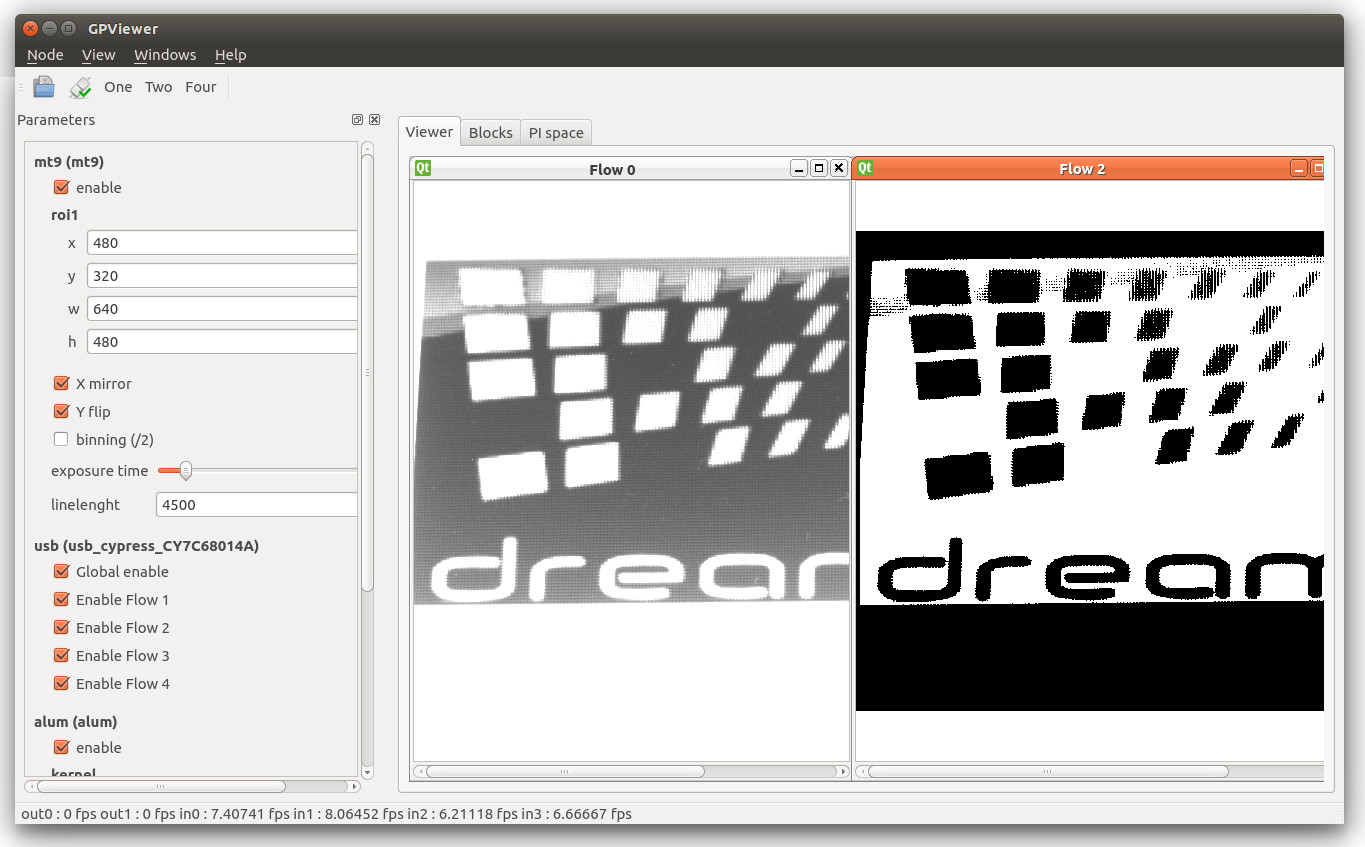
\includegraphics[scale=0.32]{gpviewer_mainwindows_threshold.jpg}
\caption{First windows of gpviewer to choose your camera}
\end{figure}

\subsection{Process with dynamic parameters}
In this section, we will add the possibility of dynamically set the threshold during camera run with the dedicated interface.

\begin{figure}[h!]
\centering
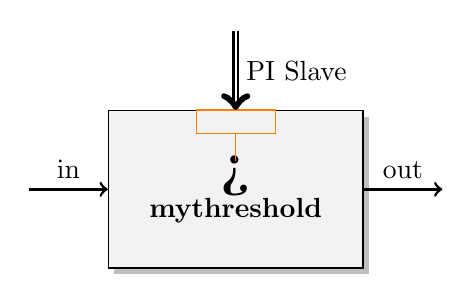
\begin{tikzpicture}[node distance=8cm]

\tikzset{blocstyle/.style={block,rectangle,minimum height=2cm,text width=2.5cm}};

% blocks
\node[blocstyle,minimum height=2cm,text width=3cm] (process1) {\textbf{\huge{>}} \\ \textbf{mythreshold}};
\draw[color=orange] ([xshift=-0.5cm]process1.north) rectangle ([xshift=0.5cm,yshift=-0.3cm]process1.north);
\draw[color=orange] ([yshift=-0.3cm]process1.north) -- ([yshift=-0.65cm]process1.north);

\path[connect,<-,double] (process1.north) -- node[right]{PI Slave} ++(0,1cm);
\path[connect,->] (process1.east) -- node[above]{out} ++(1,0);
\path[connect,<-] (process1.west) -- node[above]{in} ++(-1,0);

\end{tikzpicture}
\caption{Threshold process block with an internal register externally driven}
\end{figure}

Return in the process definition directory and create a property to set the threshold value of type int
\begin{sample}
> cd mythreshold \\
> \textbf{gpproc addproperty} -n threshold -t int
\end{sample}

A property is a high level system (API, sofware, ...) and does not have any sense to the hardware level. At the low level, the only system that could be dynamically changed, is register. A parameter is set by default as dynamic register, you just need to set a relative address and link it to the high level property with a property map expression. A property map could be expressed as a JavaScript expression and so could be very complex with conditional statements and/or mathematical functions. Here the property map is a simple link by direct value.\\

Add the register `threshold\_reg' with a relative address set to 1 and link the property value
\begin{sample}
> \textbf{gpproc addparam} -n threshold\_reg -r 1 -m threshold.value \\
Warning (1) : Your relative adress is greater than the range of relative address (0 bits). \\
Please specify a new PI size address with : \\
gpproc setpisizeaddr -v 2
\end{sample}

Set the size of PI address bus to 2 bits
\begin{sample}
> \textbf{gpproc setpisizeaddr} -v 2
\end{sample}

Generate template in the directory hdl and add the slave block
\begin{sample}
> \textbf{gpproc generate} -o hdl \\
mythreshold.vhd generated\\
mythreshold\_slave.vhd generated\\
mythreshold\_process.vhd generated\\
> \textbf{gpproc addfile} -p hdl/mythreshold\_slave.vhd -t vhdl -g hdl
\end{sample}

A new component mythreshold\_slave.vhd is generated because your process block have a PI slave interface. The new structure of components generated is described on this figure.

\begin{figure}[h!]
\centering
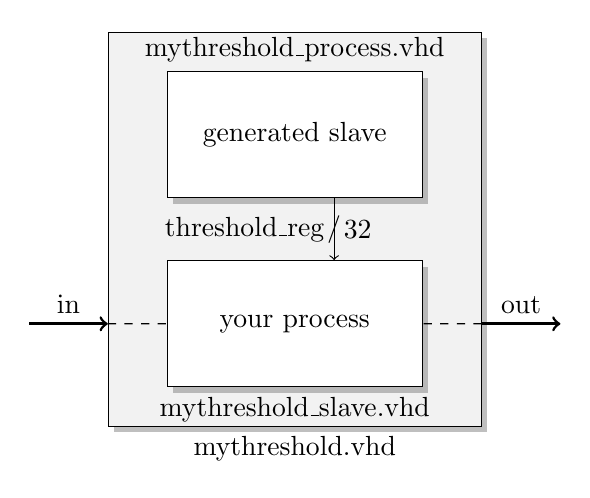
\begin{tikzpicture}[node distance=8cm]

\tikzset{blocstyle/.style={block,rectangle,minimum height=1.5cm,text width=2.5cm}};

% blocks
\node[blocstyle,minimum height=5cm,text width=4.5cm,label={below:mythreshold.vhd}] (process1) {};
\node[blocstyle,minimum height=1.6cm,text width=3cm,fill=white,label={above:mythreshold\_process.vhd}] at(0,1.2) (process1slave) {generated slave};
\node[blocstyle,minimum height=1.6cm,text width=3cm,fill=white,label={below:mythreshold\_slave.vhd}] at(0,-1.2) (process1proc) {your process};

\path[connect,->] ([yshift=-1.2cm]process1.east) -- node[above]{out} ++(1,0);
\path[connect,<-] ([yshift=-1.2cm]process1.west) -- node[above]{in} ++(-1,0);
\path[draw,dashed] ([yshift=-1.2cm]process1.east) -- (process1proc);
\path[draw,dashed] ([yshift=-1.2cm]process1.west) -- (process1proc);

\path[draw,->] ([xshift=0.5cm]process1slave.south) -- node[left]{threshold\_reg} node{/} node[right]{32} ([xshift=0.5cm]process1proc.north);

\end{tikzpicture}
\caption{Details on flow connexion}
\end{figure}

To enable the threshold value that could change dynamically, get the `threshold\_reg' register value to compare with the pixel value insted of a constant value in \texttt{threshold\_process.vhd}:
\begin{lstlisting}[frame=single]
	if(in_dv='1' and in_fv='1') then
		if(in_data >= threshold_reg(IN_SIZE-1 downto 0)) then
			out_data <= (others => '1');
		else
			out_data <= (others => '0');
		end if;
	end if;
\end{lstlisting}

Test it
\begin{sample}
> cd .. \\
> make generate compile send view
\end{sample}

\end{document}
